\begin{figure}[h!]
\centering
\caption{Deuda Neta del GNC}
\label{fig:Deuda}
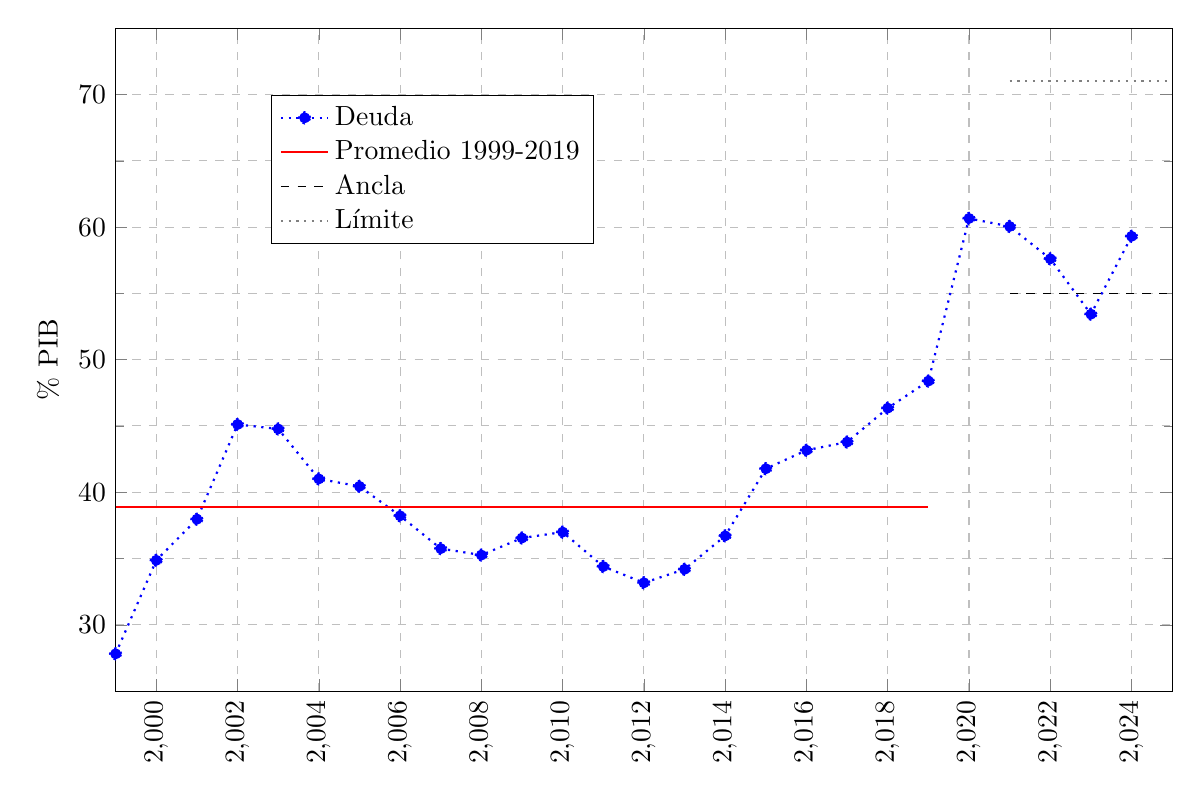
\begin{tikzpicture}
\begin{axis}[
    width=15cm, height=10cm,
    %title={Deuda Neta del GNC (\% PIB)},
    %xlabel={A\~nos},
    ylabel={\% PIB},
    ymin=25, ymax=75,
    xmin=1999, xmax=2025,
    grid=major,
    grid=both,
    grid style=dashed,
    minor y tick num=1,    
    x tick label style={rotate=90, anchor=east},
    legend style={at={(0.3,0.9)}, anchor=north},
    legend cell align={left}
]
% Deuda Neta data
\addplot[dotted, thick, blue, mark=*] table {
1999	27.81072274
2000	34.86638249
2001	37.96293129
2002	45.11098557
2003	44.77327082
2004	41.00413656
2005	40.44297265
2006	38.21961319
2007	35.74718648
2008	35.26112974
2009	36.54701602
2010	36.9931066
2011	34.39514942
2012	33.16828394
2013	34.18757347
2014	36.70888496
2015	41.77236929
2016	43.167005
2017	43.78554157
2018	46.34371284
2019	48.38488116
2020	60.65239624
2021	60.04873665
2022	57.60327227
2023	53.43060577
2024	59.30508886
};
\addlegendentry{Deuda}
% Promedio 1999-2019
\addplot[thick, red] coordinates {(1999,38.9) (2019,38.9)};
\addlegendentry{Promedio 1999-2019}
% Ancla 55%
\addplot[dashed, black] coordinates {(2021,55) (2025,55)};
\addlegendentry{Ancla}
% Limite 71%
\addplot[dotted, thick, gray] coordinates {(2021,71) (2025,71)};
\addlegendentry{L\'{i}mite}
\end{axis}
\end{tikzpicture}
\vspace{1cm}
\footnotesize{\textit{Fuente: Elaboración propia con base el saldo de la deuda del GNC, Ministerio de Hacienda.}}
\end{figure}
